%%%%%%%%%%%%%%%%%%%%%%%%%%%%%%%%%%%%%%%%%%%%%%%%%%%%%%%%%%%%%%%%%%%%%%
%%                  Fabio Pisaruk
%%
%%%%%%%%%%%%%%%%   Feito entre:  06/09/2007 a ????????    %%%%%%%%%%
%%%%%%%%%%%%%%%%%%%%%%%%%%%%%%%%%%%%%%%%%%%%%%%%%%%%%%%%%%%%%%%%%%%%%%
%\documentclass{amsart}

\documentclass[12pt]{amsart}

%% Escrevendo em portugu�s:
\usepackage[brazil]{babel}
\usepackage[latin1]{inputenc}
\usepackage[dvips]{graphicx,psfrag}
\usepackage{multicol}
\usepackage{enumerate}


%%%%%%%%%%%%%%%%%%%%%%%%%%%%%%%%%%%%%%%%%%%%%%%%%%%%%%%%%%%%%%%%%%%%%%
\renewcommand{\contentsname}{2.\enspace �ndice}
\renewcommand{\refname}{Bibliografia}
\renewcommand{\datename}{\textit{Data}:}
\makeatletter 
\renewcommand{\l@subsection}{\@tocline{2}{1pt}{2pc}{5pc}{}}
\makeatother
\setcounter{tocdepth}{2}

%% definicao personalizadamy
\usepackage{./estilo/estilo}


%%%%%%%%%%%%%%%%%%%%%%%%%%%%%%%%%%%%%%%%%%%%%%%%%%%%%%%%%%%%%%%%%%%%%%
%% Floating package
\usepackage{floatflt,epsfig,epsf}

%%%%%%%%%%%%%%%%%%%%%%%%%%%%%%%%%%%%%%%%%%%%%%%%%%%%%%%%%%%%%%%%%%%%%%
%% Dimens�o da p�gina
%\setlength{\topmargin}{-1.0cm}
%\setlength{\textheight}{22.0cm}
%\setlength{\textwidth}{15.0cm}

%\setlength{\parskip}{.5pc}
\setlength{\paperwidth}{216mm}
\setlength{\paperheight}{279mm}
\setlength{\textwidth}{150mm}
\setlength{\textheight}{220mm}
\setlength{\topmargin}{0cm}
 
% margens impar e par da pagina
%\setlength\oddsidemargin{.2cm}  
%\setlength\evensidemargin{.2cm}  
\setlength\oddsidemargin{.6cm}  
\setlength\evensidemargin{.6cm}  

%%%%%%%%%%%%%%%%%%%%%%%%%%%%%%%%%%%%%%%%%%%%%%%%%%%%%%%%%%%%%%%%%%%%%%
\newcommand{\fimprova}{
\hspace*{\fill}
\rule{0.15cm}{0.3cm}
}
%%%%%%%%%%%%%%%%%%%%%%%%%%%%%%%%%%%%%%%%%%%%%%%%%%%%%%%%%%%%%%%%%%%%%%


\begin{document}
%%%%%%%%%%%%%%%%%%%%%%%%%%%%%%%%%%%%%%%%%%%%%%%%%%%%%%%%%%%%%%%%%%%%%%
\title[$k$-caminhos m�nimos]% 
{$k$-caminhos m�nimos}
\author{F�bio Pisaruk}
\dedicatory{\small {\rm Orientador:} {\rm Jos� Coelho de Pina}} 
\address{Instituto de Matem�tica e Estat�stica, Universidade de S�o Paulo, Rua
  do Mat�o 1010, 05508--900~S�o Paulo, SP}
\email{pisaruk@ime.usp.br}
\keywords{caminhos m�nimos, otimiza��o combinat�ria}
\date{\today}
%%%%%%%%%%%%%%%%%%%%%%%%%%%%%%%%%%%%%%%%%%%%%%%%%%%%%%%%%%%%%%%%%%%%%%
\begin{abstract}
Neste projeto fazemos um esbo�o geral de uma disserta��o de mestrado que
pretende estudar o algoritmo desenvolvido por Katoh, Ibaraki e Mine de gera��o de $k$-caminhos
m�nimos sem circuitos em grafos n�o-orientados com custos n�o-negativos, bem como algumas implementa��es deste.
\end{abstract}
%%%%%%%%%%%%%%%%%%%%%%%%%%%%%%%%%%%%%%%%%%%%%%%%%%%%%%%%%%%%%%%%%%%%%%
\maketitle
%%%%%%%%%%%%%%%%%%%%%%%%%%%%%%%%%%%%%%%%%%%%%%%%%%%%%%%%%%%%%%%%%%%%%%
%\input{} 
%%%%%%%%%%%%%%%%%%%%%%%%%%%%%%%%%%%%%%%%%%%%%%%%%%%%%%%%%%%%%%%%%%%%%%
%\newpage
\tableofcontents  
%%%%%%%%%%%%%%%%%%%%%%%%%%%%%%%%%%%%%%%%%%%%%%%%%%%%%%%%%%%%%%%%%%%%%%
\setcounter{section}0

\newpage
\section{Introdu��o}

\par
\begin{floatingfigure}[l]{30mm}
\begin{center}
  \psfrag{s}{$s$}
  \psfrag{t}{$t$}
  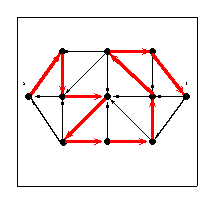
\includegraphics{./figs/rede}
\end{center} 
\end{floatingfigure}
\noindent


Uma certa empresa de telecomunica��es, cujo nome real n�o ser�
citado por raz�es de confidencialidade, mas que para nossa
comodidade ser� chamada de TeleMax, fornece linhas de transmiss�o
aos seus clientes de modo que estes possam, por exemplo, ligar-se
�s suas filiais por linhas privadas.
Para tal, conta com uma infra-estrutura (rede) bastante complexa
compreendendo cabos e diversos equipamentos de jun��o.  Esta rede
� ``full-duplex'', ou seja, possui passagem de dados em ambos os
sentidos.  Para entender o processo de fornecimento de linhas de
transmiss�o, passemos a um breve exemplo.  A empresa SoftSOF
possui duas sedes, uma em Santos e outra em Fernand�polis e, a
fim de diminuir gastos com locomo��o e hospedagem, necessita de
um rede que conecte as duas sedes com uma qualidade tal que
permita que teleconfer�ncias sejam realizadas.  Ela solicita
ent�o a TeleMax um ``link`` de 512 Mbits ligando as suas sedes.
A TeleMaxi n�o possui uma liga��o direta entre as duas cidades,
entretanto possui uma liga��o que passa por S�o Jose do Rio
Preto, ou seja, um caminho Santos - S�o Jos� Do Rio Preto -
Fernand�polis.  Infelizmente este link s� disp�e de 256 Mbits.
Observando sua infra-estrutura, descobre que existe um outro
caminho: Santos - S�o Paulo - Fernand�polis, tamb�m com
capacidade de 256MBits.  Pronto. A TeleMax pode fornecer o link
requerido pela SoftSOF, bastando para isso utilizar os dois
caminhos acima descritos que totalizam 512 MBits.

\par
\begin{figure}[htbp]
\begin{center}
  \psfrag{Santos }{fiSantos}
  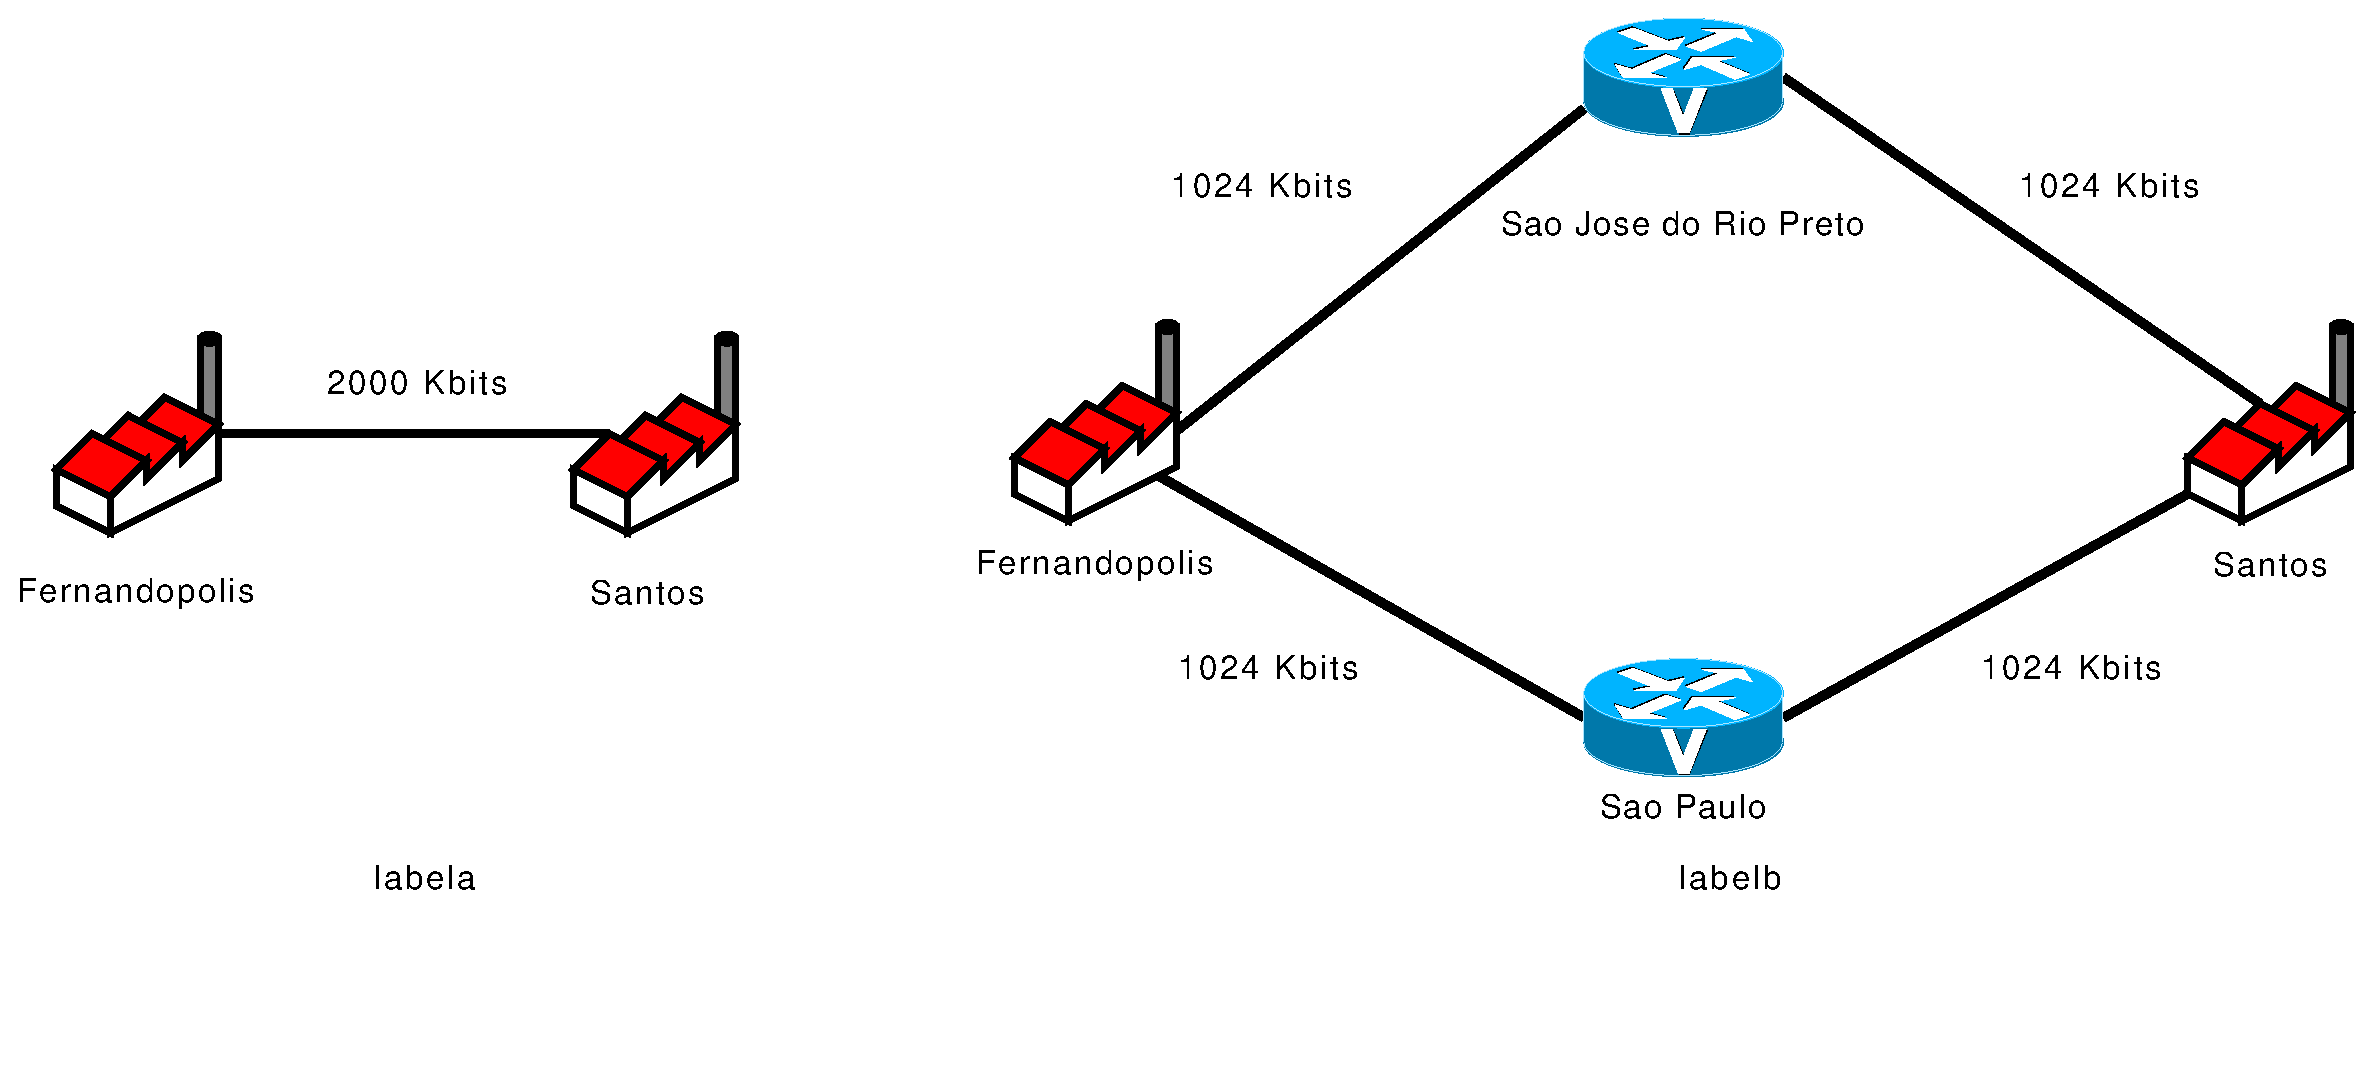
\includegraphics[width=1\textwidth]{./figs/introducaoTeleMax}
\end{center} 
\end{figure}
\noindent
Vamos a algumas considera��es relevantes. O custo de um caminho � fun��o da quantidade de equipamentos usada e n�o da dist�ncia total dos cabos que o comp�e.
Isto se deve ao custo elevado dos equipamentos se comparados aos dos cabos. Assim, passa a ser melhor utilizar uma liga��o que percorre uma dist�ncia 
maior mas que passe por um n�mero menor de equipamentos, do que uma com menor dist�ncia mas que se utiliza de mais equipamentos.


A justificativa para a gera��o de diversos caminhos no lugar de apenas um est� relacionada � capacidade de transmiss�o dispon�vel por cabo.
A motiva��o para a gera��o de caminhos m�nimos, ou seja, com utiliza��o m�nima de equipamentos, requer uma explica��o mais detalhada.
At� agora fomos simplistas ao tratarmos das rela��es entre cabos e equipamentos como se um equipamento se ligasse a apenas um cabo.
Na verdade, cada equipamento se liga a um grande n�mero de cabos. 
Assim, podemos ter diversos caminhos entre dois equipamentos, um para cada cabo.
A fim de utilizarmos bem os recursos da rede, � interessante que o menor n�mero de equipamentos esteja alocado para cada cliente pois, 
desta maneira, um n�mero maior de liga��es poder� ser oferecido pela TeleMax.
Embora a utiliza��o do menor n�mero poss�vel de equipamentos para cada cliente n�o seja
suficiente para garantir que a rede esteja sendo utilizada de maneira eficiente, 
n�o nos importaremos com isto neste trabalho.
Feitas as devidas considera��es, vamos agora justificar a automa��o do processo.


Imagine levar � cabo o processo de fornecimento de linhas, chamado a partir de agora de provisionamento, manualmente.
Podemos salientar alguns problemas da abordagem manual.
Devido �s dimens�es da rede, o operador respons�vel levar� muito tempo para obter uma lista de caminhos entre os pontos.
Durante o tempo em que o operador gasta analisando a rede, esta poder� ter sofrido altera��es as quais n�o serao levadas em conta por ele.
Al�m disso, sabemos como as pessoas s�o suscetiveis a falhas, ainda mais quando expostas a atividades ma�antes e repetitivas.
Por conta destes fatores, a TeleMax sentiu a necessidade de uma ferramenta computacional que gerasse de maneira r�pida e confi�vel 
uma s�rie de caminhos entre dois pontos da sua rede.

Modelamos o problema acima da seguinte maneira.
Consideramos a rede como um grafo n�o-orientado, por ser full-duplex, onde as arestas s�o representadas pelos cabos e os v�rtices pelos equipamentos.
A ferramenta, tinha como n�cleo o algoritmo desenvolvido Katoh, Ibaraki e Mine (KIM), 
de gera��o de caminhos m�nimos.
Os caminhos de mesmo custo, ou seja, que se utilizam de igual quantidade de equipamentos, s�o posteriormente reordenados crescentemente pela dist�ncia total 
percorrida por seus cabos.
Esta disserta��o trata do algoritmo KIM, 
que gera $k$-caminhos m�nimos sem circuitos em grafos n�o-orientados. 
Embora algoritmos para tal sejam de interesse te�rico,
� interessante observar que foi uma aplica��o pr�tica demandada por uma necessidade surgida no �mbito empresarial que nos levou ao estudo do mesmo.
 


Otimiza��o combinat�ria � um campo da matem�tica aplicada que usa t�cnicas de combinat�ria, programa��o matem�tica e
teoria de algoritmos para resolver problemas em otimiza��o sobre estruturas discretas. 

Problemas em otimiza��o combinat�ria t�m sido um t�pico central para a evolu��o de algoritmos e da teoria de complexidade computacional.
Pesquisadores t�m apresentado muitas id�ias criativas para o projeto de algoritmos eficientes baseados em conceitos e resultados na �rea. 
M�todos desenvolvidos para problemas em fluxos em redes, como o primal-dual, t�m se mostrado muito �teis no projeto e an�lise de uma variedade de
algoritmos para problemas em outros dom�nios. 
Muitas das id�ias inovadoras t�m se baseado em um conjunto n�o muito grande de princ�pios  comuns que s�o
simultaneamente simples e poderosos (como \textit{scaling}).

%% Neste projeto pretendemos estudar algumas das ferramentas mais
%% fundamentais em otimiza��o combinat�ria. Desejamos
%% analisar e implementar algoritmos para diversos problemas
%% cl�ssicos, principalmente em fluxos em redes e
%% emparelhamentos.  O nosso guia nessa jornada ser� o livro de
%% Ahuja, Magnanti e Orlin~\cite{ahuja:netflows}, com o livro de
%% Cook, Cunningham, Pulleyblank e
%% Schrijver~\cite{cook:co-1998} como um guia secund�rio. Para
%% os t�picos mais te�ricos consultaremos os livros de
%% Schrijver~\cite{schrijver:tilp-1986,schrijver:cope-2003}.
%% Criaremos um s�tio na internet para armazenar todas as
%% implementa��es, textos e anima��es produzidas durante a
%% execu��o do projeto.
 

\newpage
\input{02-problema}

%\newpage
%\input{03-...}

%\newpage
%\input{04-...}

%\newpage
%\input{05-...}

%\newpage
%\input{06-}

%\newpage
%\input{08-proposta}



%%%%%%%%%%%%%%%%%%%%%%% Bibliografia %%%%%%%%%%%%%%%%%%%%%%%%%%%%%%%%%
%\cite{*}
\newpage 
\bibliographystyle{./bib/joseplain} 
\bibliography{./bib/refs}

\end{document}












